The application architecture consists of three distinct components, as
presented in \Cref{fig:tool-architecture}. The frontend is responsible for the
interface between the tool logic and the user. The tool domain contains
adapters for each individual tool and the tool runtime, which receives the
monolithic input and generates the candidate microservices. The backend serves
as a bridge between the frontend, the database of available tools, and the tool
domain.

\begin{figure*}[!htb]
  \caption{Application architecture}
  \label{fig:tool-architecture}
  \centering
  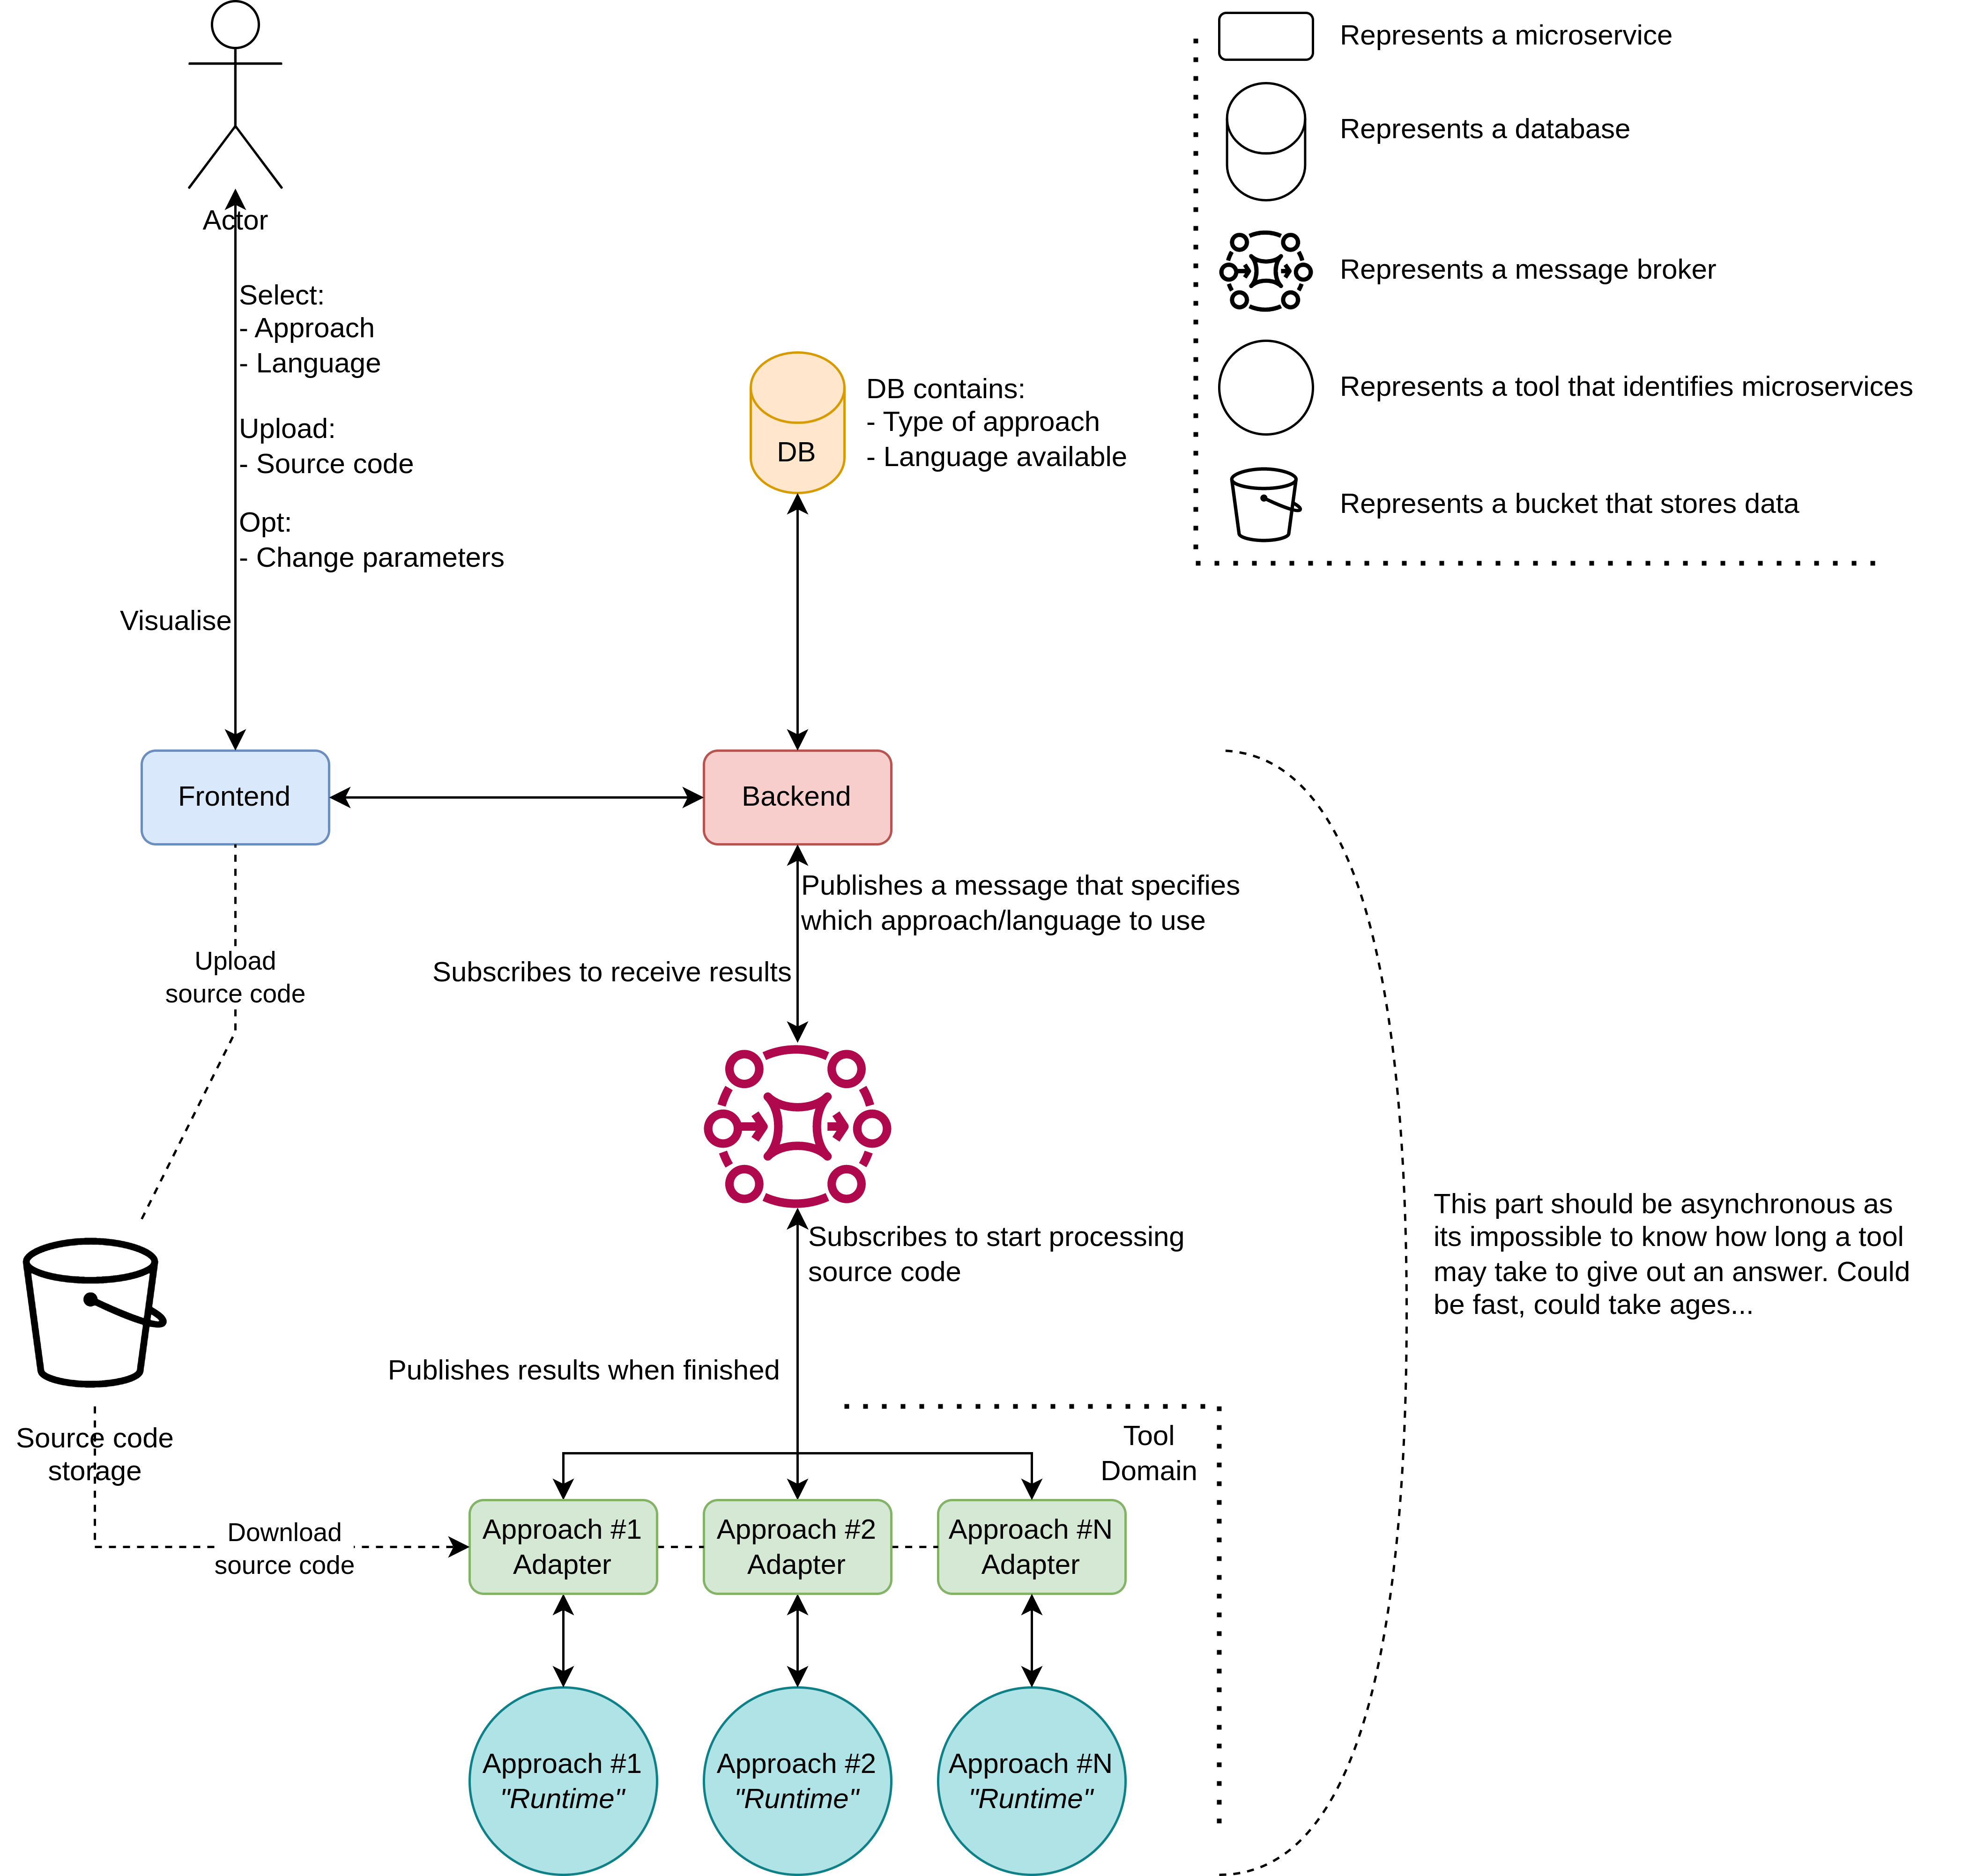
\includegraphics[width=\textwidth]{thesis-architecture.drawio}
\end{figure*}

The main role of the backend component is to initiate jobs and notify the
frontend when a given job has been completed. A job consists of the process of
identifying microservices from a given monolithic input, which is then
completed when the output containing the identified microservices is produced.
To avoid potential bottlenecks when multiple jobs are run concurrently, the
backend does not perform these tasks directly but rather delegates them to the
individual tools, therefore acting like a bridge.

In the tool domain, the purpose of the adapter is to provide a consistent
interface for interacting with the tool runtime, regardless of the specific
input and output formats that it uses. This is important because different
tools may accept different inputs and produce different outputs, such as JSON
or raw code. By using an adapter to translate between these formats, it becomes
easier to process the inputs and outputs of the tool and integrate them with
the overall tool logic. The tool runtime receives the monolithic input and
generates the candidate microservices, while the adapter serves as a
``middleman'' between the tool runtime and the other components of the
architecture.

Given that the tasks performed by the tool runtime component are asynchronous,
the communication between the tool runtime and the backend cannot be based on
synchronous HTTP request-response cycles. Instead, we will use a message queue
to connect the two components, with the use of message brokers. The backend
will send a message to initiate a job, which will be picked up by the
appropriate adapter and executed by the tool runtime. Once the job is
completed, the tool runtime will send another message to the backend to
indicate that it is finished. This approach allows us to process multiple jobs
concurrently and avoid potential bottlenecks in the communication between the
tool runtime and the backend.
